
\documentclass[11pt,a4paper]{article}

\usepackage[utf8]{inputenc}
\usepackage[T1]{fontenc}
\usepackage{lmodern}
\usepackage{amsmath,amssymb}
\usepackage{graphicx}
\usepackage{caption}
\usepackage{subcaption}
\usepackage{booktabs}
\usepackage{geometry}
\usepackage{hyperref}

\geometry{margin=2.5cm}
\graphicspath{{../figures/}}

\begin{document}

\begin{titlepage}
    \centering
    \vspace*{0.28\textheight}

    {\LARGE\bfseries Empirical Stability of \par}
    {\LARGE\bfseries Least Squares and \par}
    {\LARGE\bfseries Ridge Regression\par}

    \vspace{1.5cm}

    \vfill
\end{titlepage}

\section*{Declaration}

I declare that this material, which I now submit for assessment, is entirely my own work and has not been taken from the work of others, save and to the extent that such work has been cited and acknowledged within the text of my work. I understand that plagiarism, collusion, and copying are grave and serious offences in the university and accept the penalties that would be imposed should I engage in plagiarism, collusion or copying. This assignment, or any part of it, has not been previously submitted by me or any other person for assessment on this or any other course of study.

\newpage

\section{Introduction}

This project studies how \textbf{Least Squares} and \textbf{Ridge Regression} behave when the training set is slightly changed. In addition to prediction error, we also consider the \textbf{stability} of the two methods by looking at how much the predictions change when one observation is removed from the training data~\cite{bousquet2002stability}.

The goal is to understand when the regularization used by Ridge can make the model less sensitive to the training data, and what effect this has on prediction accuracy.

To make the comparison clearer, the analysis starts with synthetic data, using both independent and correlated predictors. The effect of sample size is then studied separately. Finally, the same methods are applied to the real \emph{Seoul Bike Sharing Demand} dataset to see whether the behavior observed in the controlled experiments also appears in a more realistic setting.

The experiments are repeated with different seeds, and Ridge is tested with different values of the regularization parameter $\lambda$. This avoids drawing conclusions from a single random train--test split and makes it possible to study the \textbf{trade-off between stability and prediction accuracy} as the strength of regularization changes.

\section{Methodology}

\subsection{Least Squares and Ridge Regression}
We start with a linear regression model, where the response variable is represented as a linear combination of the explanatory variables. Let $X$ be the matrix of predictors, $y$ the vector of observed response values, and $\beta$ the vector of coefficients. The predictions can be written as

\begin{equation}
    \hat{y} = X\hat{\beta}.
\end{equation}

In \textbf{Least Squares}, the coefficients are chosen by minimizing the sum of squared errors between the observed and predicted values:

\begin{equation}
    \hat{\beta}_{LS}
    = \arg\min_{\beta} \|y-X\beta\|_2^2.
\end{equation}

When some explanatory variables contain very similar information, small changes in the data can lead to large changes in the estimated coefficients.

\textbf{Ridge Regression}, instead, adds an $L_2$ penalty to the objective function~\cite{hoerl1970ridge}:

\begin{equation}
    \hat{\beta}_{Ridge}
    = \arg\min_{\beta}
    \left\{
    \frac{1}{n}\|y-X\beta\|_2^2 + \lambda\|\beta\|_2^2
    \right\}.
\end{equation}

The parameter $\lambda \geq 0$ controls the strength of regularization. If $\lambda=0$, the problem is the same as Least Squares. As $\lambda$ increases, large coefficients are penalized more strongly. Ridge therefore introduces some bias in order to reduce the variability of the model.

The intercept is not penalized. In the code, Ridge is estimated by centering $X$ and $y$ and applying the penalty only to the coefficients of the explanatory variables. In the real dataset, the features are standardized because the Ridge penalty acts directly on coefficient size, and variables measured on very different scales would otherwise be penalized in an uneven way.

\subsection{Empirical Stability Measure}

To compare the sensitivity of the two algorithms, a \emph{leave-one-out} procedure is used. For each training set, the model is first fitted using all available observations and its predictions are computed on the test set. Then, one observation at a time is removed, the model is fitted again, and the new predictions on the same test set are compared with those of the full model.

Let $\hat{f}$ be the model fitted on the full training set and $\hat{f}^{(-i)}$ the model obtained after removing observation $i$. For each removed point, the mean absolute change in predictions is computed as

\begin{equation}
    S_i = \frac{1}{m}\sum_{j=1}^{m}
    \left|
    \hat{f}(x_j)-\hat{f}^{(-i)}(x_j)
    \right|,
\end{equation}

where $m$ is the number of observations in the test set. The overall measure used in the experiments is then

\begin{equation}
    S = \frac{1}{n}\sum_{i=1}^{n} S_i,
\end{equation}

where $n$ is the number of training observations considered in the leave-one-out procedure.

This measure shows how much the predictions change, on average, when one observation is removed from the training set. A small value of $S$ means that the model changes little and is therefore more stable.

\subsection{Evaluation of Predictive Performance}

Stability is studied together with predictive performance. The error measure used is the \textbf{Mean Squared Error}:

\begin{equation}
    \mathrm{MSE} = \frac{1}{m}\sum_{j=1}^{m}(y_j-\hat{y}_j)^2.
\end{equation}

It is computed separately on the training set and on the test set. The training error shows how well the model fits the data used for estimation, while the test error shows how the model performs on observations that were not used during training. To avoid data leakage, model estimation and all required transformations are based only on information from the training set.

The \textbf{generalization gap} is also considered and is defined as

\begin{equation}
    \mathrm{Gap} = \mathrm{MSE}_{test} - \mathrm{MSE}_{train}.
\end{equation}

It is used as additional information to help interpret the behavior of the model.

\section{Experiments on Synthetic Data}

The first part of the analysis uses synthetic data. This makes it possible to work in a controlled setting, where the process used to generate the response variable is known and some characteristics of the data can be changed while keeping the others fixed.

\subsection{Data Generation}

In each experiment, $n=200$ observations are generated with $p=10$ explanatory variables. The predictors are drawn from a multivariate normal distribution with mean zero. The true coefficients used to generate the response increase from 1 to 3, while the noise is drawn from a normal distribution with mean zero and standard deviation equal to 1. The response variable therefore follows the model

\begin{equation}
    y = X\beta + \varepsilon,
\end{equation}

where $\beta$ is the vector of true coefficients and $\varepsilon \sim \mathcal{N}(0,1)$. The noise term represents the part of the response that is not explained by the variables included in the model. Adding noise makes the synthetic data less perfect and more similar to a real problem.

The 200 observations are split into training and test sets, using $75\%$ of the data for training and the remaining $25\%$ for testing.

\subsection{Base and Correlated Scenarios}

Two synthetic scenarios are considered. In the first one, called \textbf{BASE}, the explanatory variables are independent and measured on the same scale. This is the simplest case and is used as a reference for the comparison with Ridge.

In the second scenario, called \textbf{CORRELATED}, a correlation of $\rho=0.8$ is introduced between the predictors. The aim is to create a setting in which the variables contain very similar information. In this case, Least Squares can become more sensitive to changes in the sample, while Ridge can benefit more from regularization. Comparing the two scenarios makes it possible to study the effect of correlation while keeping the other parts of the experiment unchanged.

For Ridge, the following values are used:

\begin{equation}
    \lambda \in \{0.001,\,0.01,\,0.1,\,1,\,10,\,100\}.
\end{equation}

This grid shows how the model behaves from very weak to very strong regularization. Small values keep Ridge close to Least Squares, while larger values show what happens when the penalty becomes too strong.

Each configuration is repeated with \textbf{20 random seeds}. In each repetition, the generated data and the train--test split change, while the experiment settings remain the same. For each metric, the mean and standard deviation over the 20 experiments are then computed, so that the conclusions do not depend on a single random realization of the data.

\subsection{Results on Synthetic Data}

The main results are summarized in Table~\ref{tab:synthetic-results}, which compares Least Squares and Ridge in the two scenarios using Test MSE and the average prediction change.

Looking at stability and prediction error separately across the different values of $\lambda$ helps show how the effect of regularization changes as the penalty becomes stronger.

\begin{table}[ht]
    \centering
    \begin{tabular}{llcc}
        \toprule
        Scenario & Model & Test MSE & Average prediction change \\
        \midrule
        BASE & Least Squares & 1.1268 & 0.0150 \\
        BASE & Ridge ($\lambda=0.01$) & 1.1219 & 0.0149 \\
        BASE & Ridge ($\lambda=0.1$) & 1.5196 & 0.0167 \\
        BASE & Ridge ($\lambda=1$) & 13.0968 & 0.0299 \\
        \midrule
        CORRELATED & Least Squares & 1.1268 & 0.0150 \\
        CORRELATED & Ridge ($\lambda=0.01$) & 1.1227 & 0.0143 \\
        CORRELATED & Ridge ($\lambda=0.1$) & 1.2478 & 0.0115 \\
        CORRELATED & Ridge ($\lambda=1$) & 5.7722 & 0.0172 \\
        \bottomrule
    \end{tabular}
    \caption{Comparison of Test MSE and average prediction change in the BASE and CORRELATED synthetic scenarios. Lower values of the second metric indicate greater stability.}
    \label{tab:synthetic-results}
\end{table}

In the BASE scenario, Ridge with small values of $\lambda$ behaves almost like Least Squares. With $\lambda=0.01$, for example, both Test MSE and average prediction change remain almost unchanged. When regularization becomes stronger, both the error and the prediction change increase. In this case, Ridge does not provide a clear advantage in terms of stability.

The CORRELATED scenario shows a different behavior. With $\lambda=0.1$, the average prediction change decreases from $0.0150$ for Least Squares to $0.0115$ for Ridge, which is a reduction of about $23\%$. Test MSE increases from $1.1268$ to $1.2478$, but the increase is still limited compared with the improvement in stability. This is the most interesting case among the synthetic experiments.

Also in the correlated scenario, too much regularization becomes harmful. With $\lambda=1$, both the error and the average prediction change increase, and the effect becomes stronger for even larger values. Overall, the results suggest that \textbf{moderate regularization can improve stability especially when the predictors are strongly correlated}, while too much regularization can worsen both stability and prediction accuracy.

\begin{figure}[ht]
    \centering
    \begin{minipage}{0.48\textwidth}
        \centering
        \includegraphics[width=\linewidth]{stability_vs_lambda_BASE.png}
    \end{minipage}\hfill
    \begin{minipage}{0.48\textwidth}
        \centering
        \includegraphics[width=\linewidth]{test_error_vs_lambda_BASE.png}
    \end{minipage}
    \caption{BASE scenario: average prediction change and Test MSE for different values of $\lambda$.}
    \label{fig:base-results}
\end{figure}

\begin{figure}[ht]
    \centering
    \begin{minipage}{0.48\textwidth}
        \centering
        \includegraphics[width=\linewidth]{stability_vs_lambda_CORRELATED.png}
    \end{minipage}\hfill
    \begin{minipage}{0.48\textwidth}
        \centering
        \includegraphics[width=\linewidth]{test_error_vs_lambda_CORRELATED.png}
    \end{minipage}
    \caption{CORRELATED scenario: average prediction change and Test MSE for different values of $\lambda$.}
    \label{fig:correlated-results}
\end{figure}

\section{Effect of Sample Size}

To understand how stability also depends on the amount of available data, an additional experiment is carried out by changing the sample size. When the training set is small, removing one observation can have a larger effect on the model. When the sample is larger, the same observation has a smaller impact.

The number of variables is kept fixed at $p=10$, while four sample sizes are considered:

\begin{equation}
    n \in \{50,\,100,\,200,\,500\}.
\end{equation}

For each value of $n$, the same $75\%$--$25\%$ train--test split is used and the experiment is repeated with 20 seeds. For Ridge, $\lambda=0.01$ is fixed, so that the effect of sample size can be studied without changing the level of regularization at the same time.

Comparing the two methods across increasing sample sizes also makes it easier to see how the prediction change decreases as more observations become available.

The results show a clear decrease in the average prediction change as $n$ increases. For Least Squares, the value goes from $0.0777$ with $n=50$ to $0.0056$ with $n=500$. Ridge follows almost the same pattern, decreasing from $0.0763$ to $0.0056$.

\begin{table}[ht]
    \centering
    \begin{tabular}{ccc}
        \toprule
        $n$ & Least Squares & Ridge ($\lambda=0.01$) \\
        \midrule
        50  & 0.0777 & 0.0763 \\
        100 & 0.0332 & 0.0329 \\
        200 & 0.0150 & 0.0149 \\
        500 & 0.0056 & 0.0056 \\
        \bottomrule
    \end{tabular}
    \caption{Average prediction change for different sample sizes. Lower values indicate greater stability.}
    \label{tab:sample-size-stability}
\end{table}

As the number of observations increases, both models become more stable. The difference between Least Squares and Ridge remains very small, which is consistent with the low value of $\lambda$ used in this experiment.

This shows that stability does not depend only on the algorithm, but also on the amount of available data. With a larger training set, removing one observation has a smaller effect on the model and therefore also on its predictions.

\begin{figure}[ht]
    \centering
    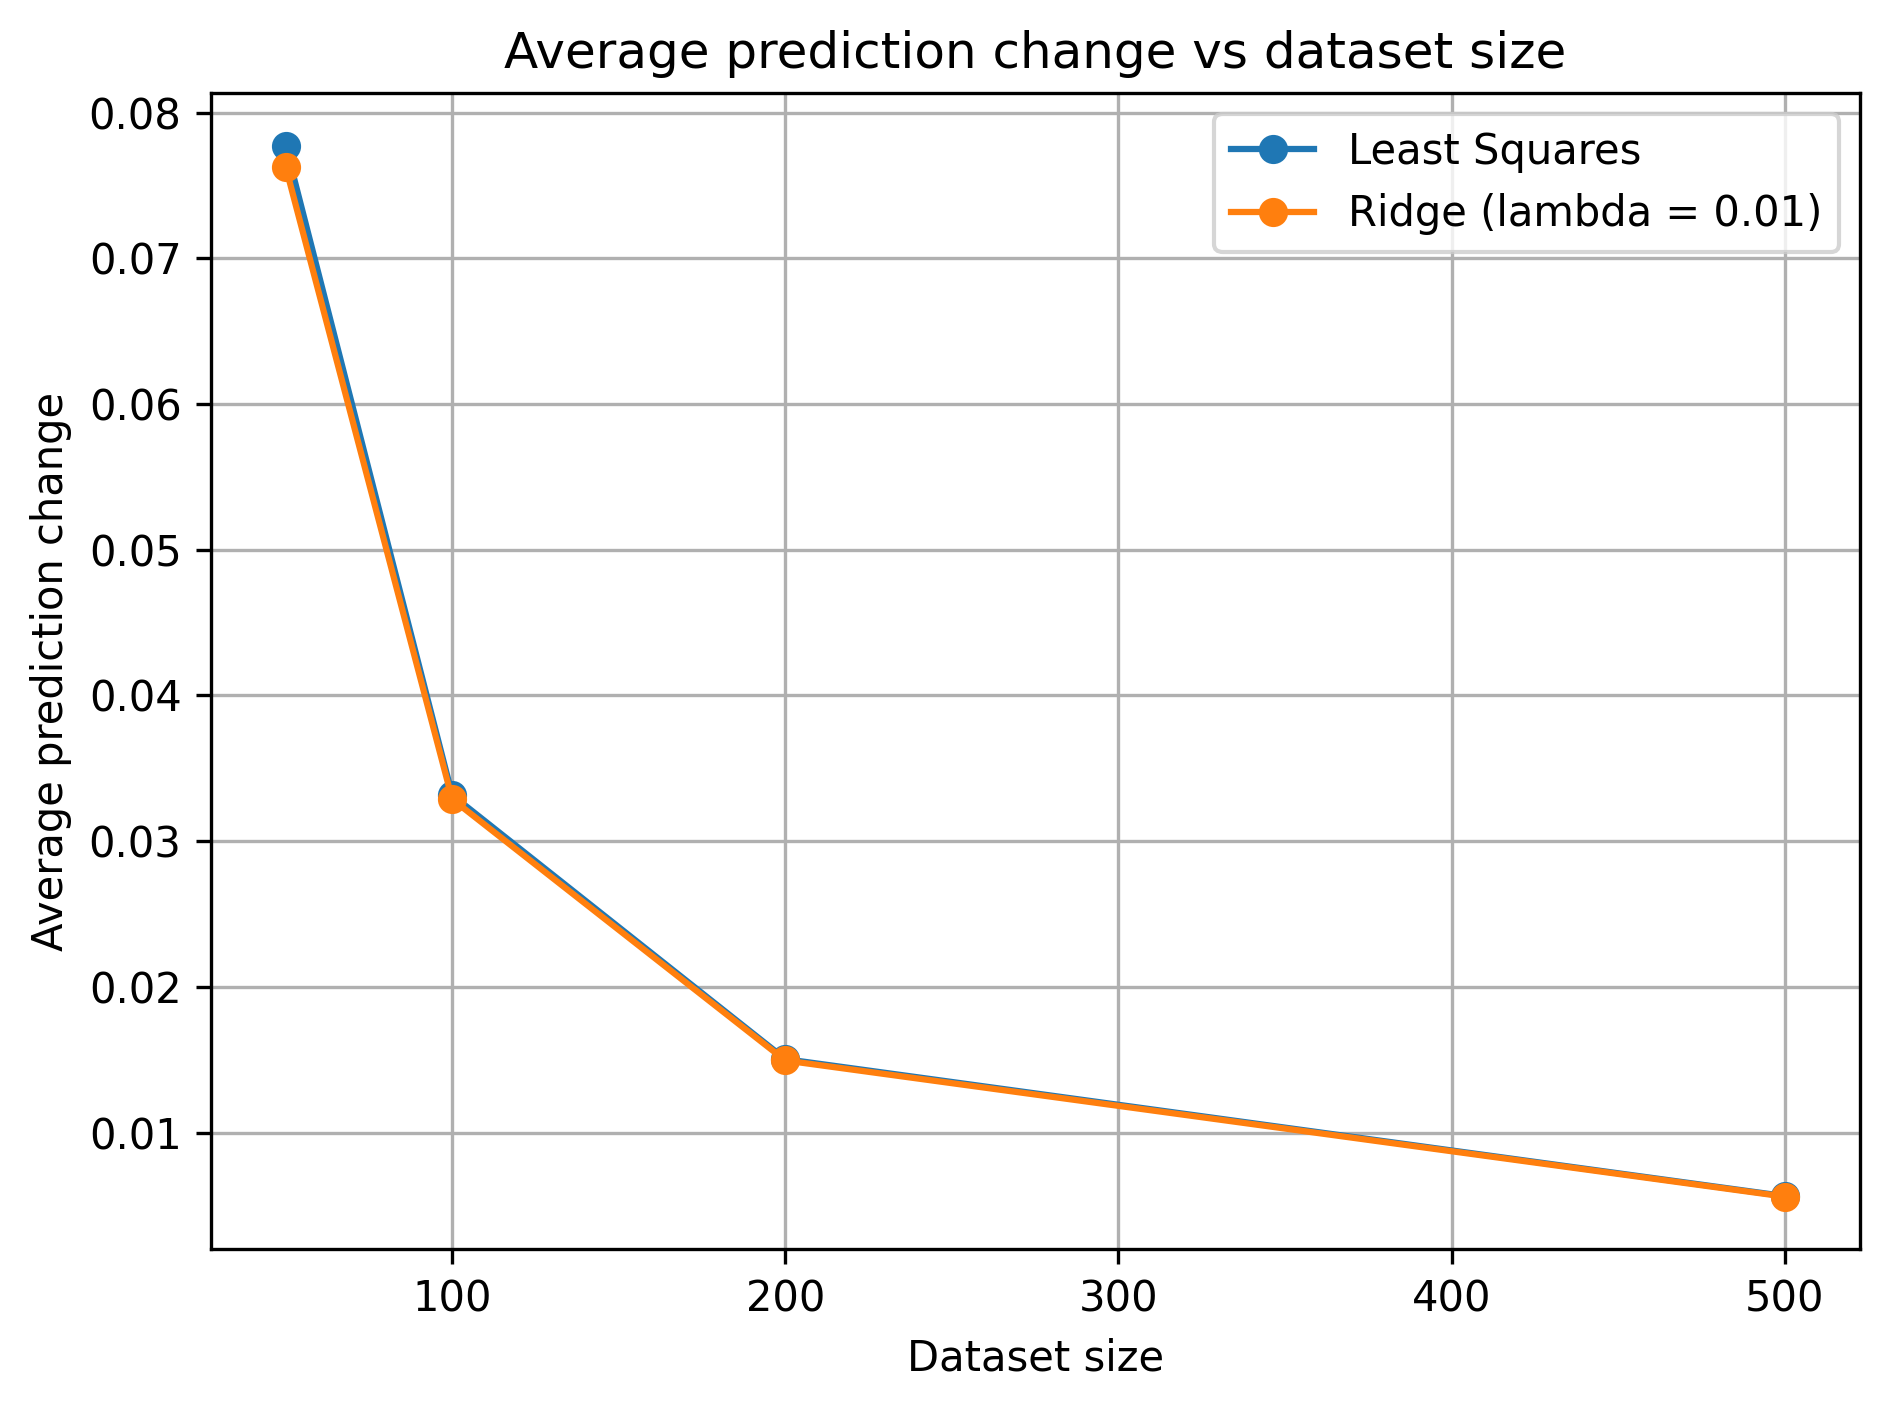
\includegraphics[width=0.50\textwidth]{stability_vs_sample_size.png}
    \caption{Effect of sample size on the average prediction change of Least Squares and Ridge Regression.}
    \label{fig:sample-size-stability}
\end{figure}


\section{Real Dataset: Seoul Bike Sharing}

\subsection{Dataset Choice and Exploration}

Finally, the analysis is applied to the \emph{Seoul Bike Sharing Demand} dataset from the UCI Machine Learning Repository~\cite{uci2020seoul}. The dataset contains 8760 observations and 14 variables and describes, on an hourly basis, the number of rented bikes together with time and weather information. The response variable is \emph{Rented Bike Count}, which is the number of bikes rented in a given hour.

Before fitting the models, a simple exploratory analysis is carried out. There are no missing values, so no imputation procedure is needed.

The exploratory analysis focuses on the distribution of the response, its relationship with time and temperature, and the correlation between numerical predictors. These aspects are useful for understanding the structure of the data before comparing Least Squares and Ridge.

The distribution of the response variable is skewed: most observations have a relatively low number of rentals, while in some hours the number of rented bikes is above 3000 (Figure~\ref{fig:target-distribution}).

The hour of the day also shows a clear relationship with demand. The average number of rentals changes during the day and is higher during the time periods linked to daily commuting (Figure~\ref{fig:rentals-hour}).

Temperature also has a generally positive relationship with the number of rentals: higher temperatures are often associated with larger values of \emph{Rented Bike Count}, although the points are quite spread out (Figure~\ref{fig:rentals-temperature}).

Finally, the correlation matrix shows some important relationships between the weather variables. In particular, temperature and dew point temperature are strongly correlated. This makes the dataset useful for the comparison with Ridge, because correlation between predictors is already present in the real data and is not created artificially (Figure~\ref{fig:seoul-correlation}).

\begin{figure}[ht]
    \centering
    \begin{subfigure}{0.48\textwidth}
        \centering
        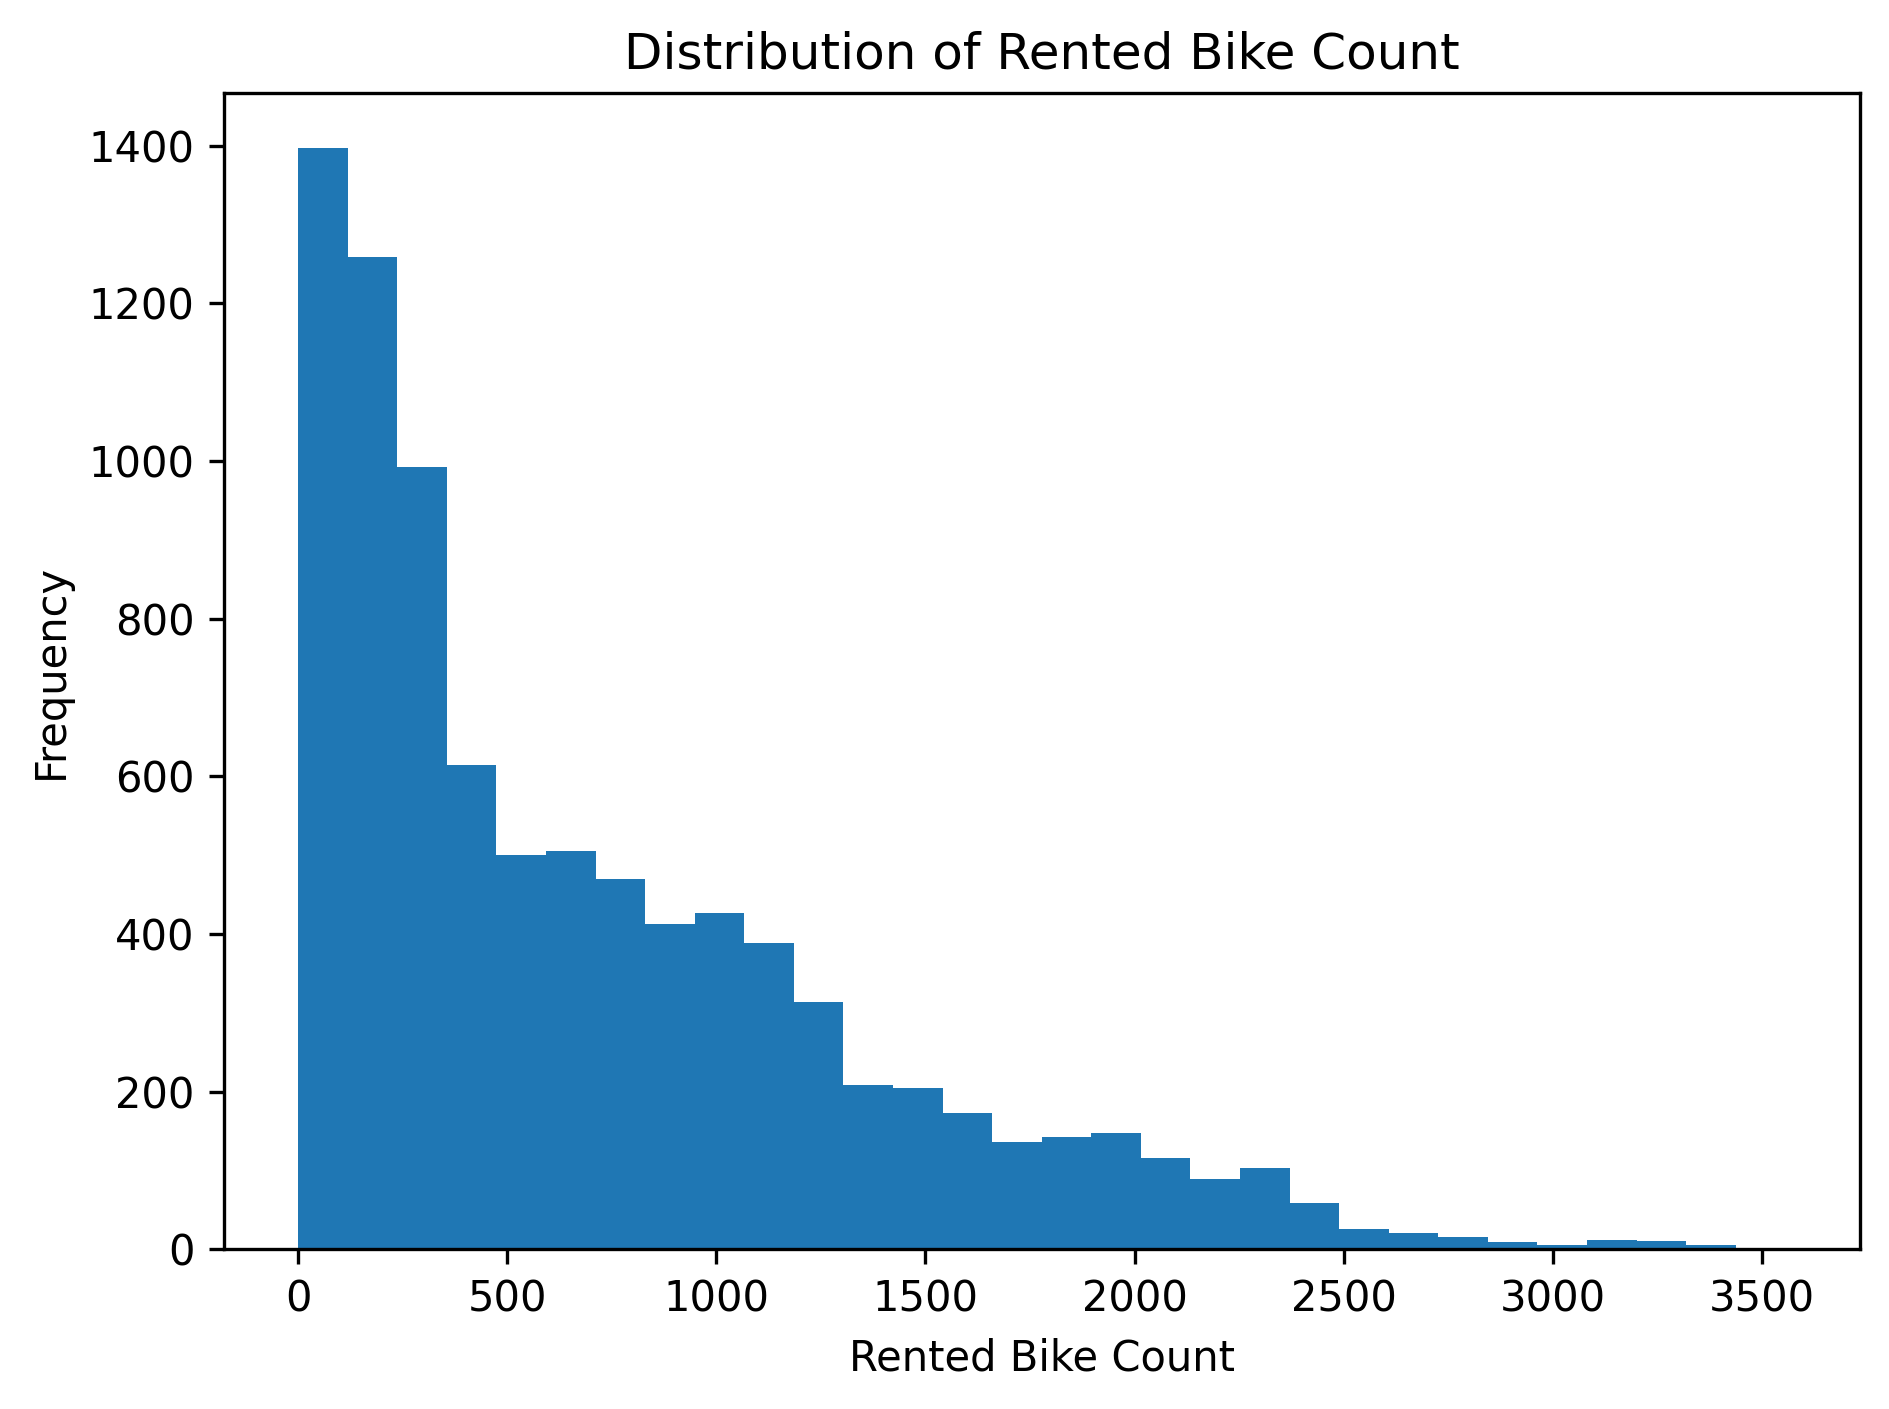
\includegraphics[width=\linewidth]{target_distribution.png}
        \caption{Distribution of \emph{Rented Bike Count}.}
        \label{fig:target-distribution}
    \end{subfigure}\hfill
    \begin{subfigure}{0.48\textwidth}
        \centering
        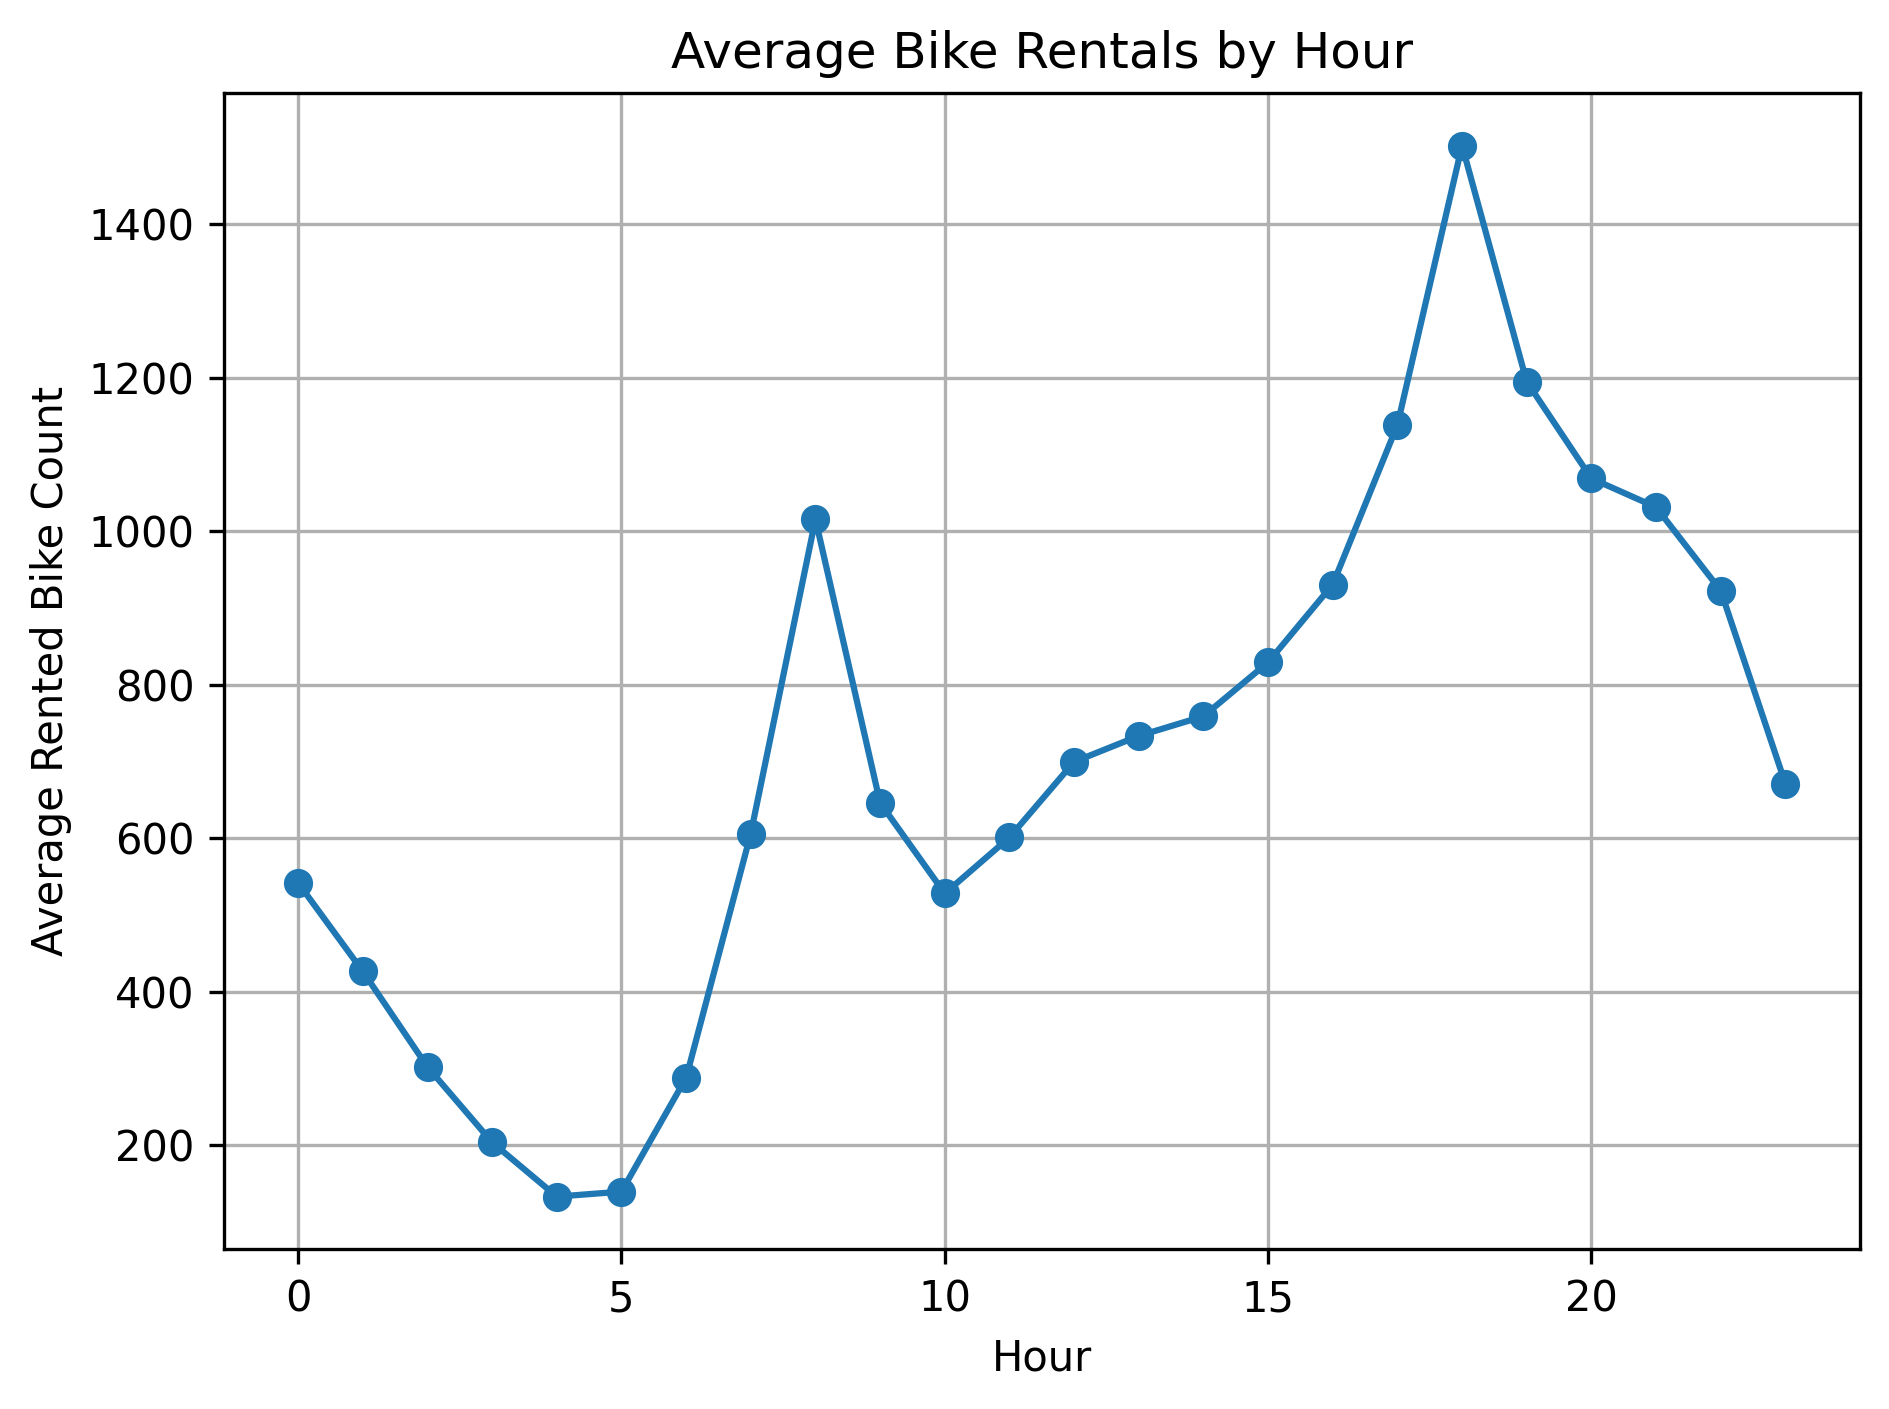
\includegraphics[width=\linewidth]{rentals_by_hour.png}
        \caption{Average number of rented bikes during the different hours of the day.}
        \label{fig:rentals-hour}
    \end{subfigure}

    \vspace{0.6cm}

    \begin{subfigure}{0.48\textwidth}
        \centering
        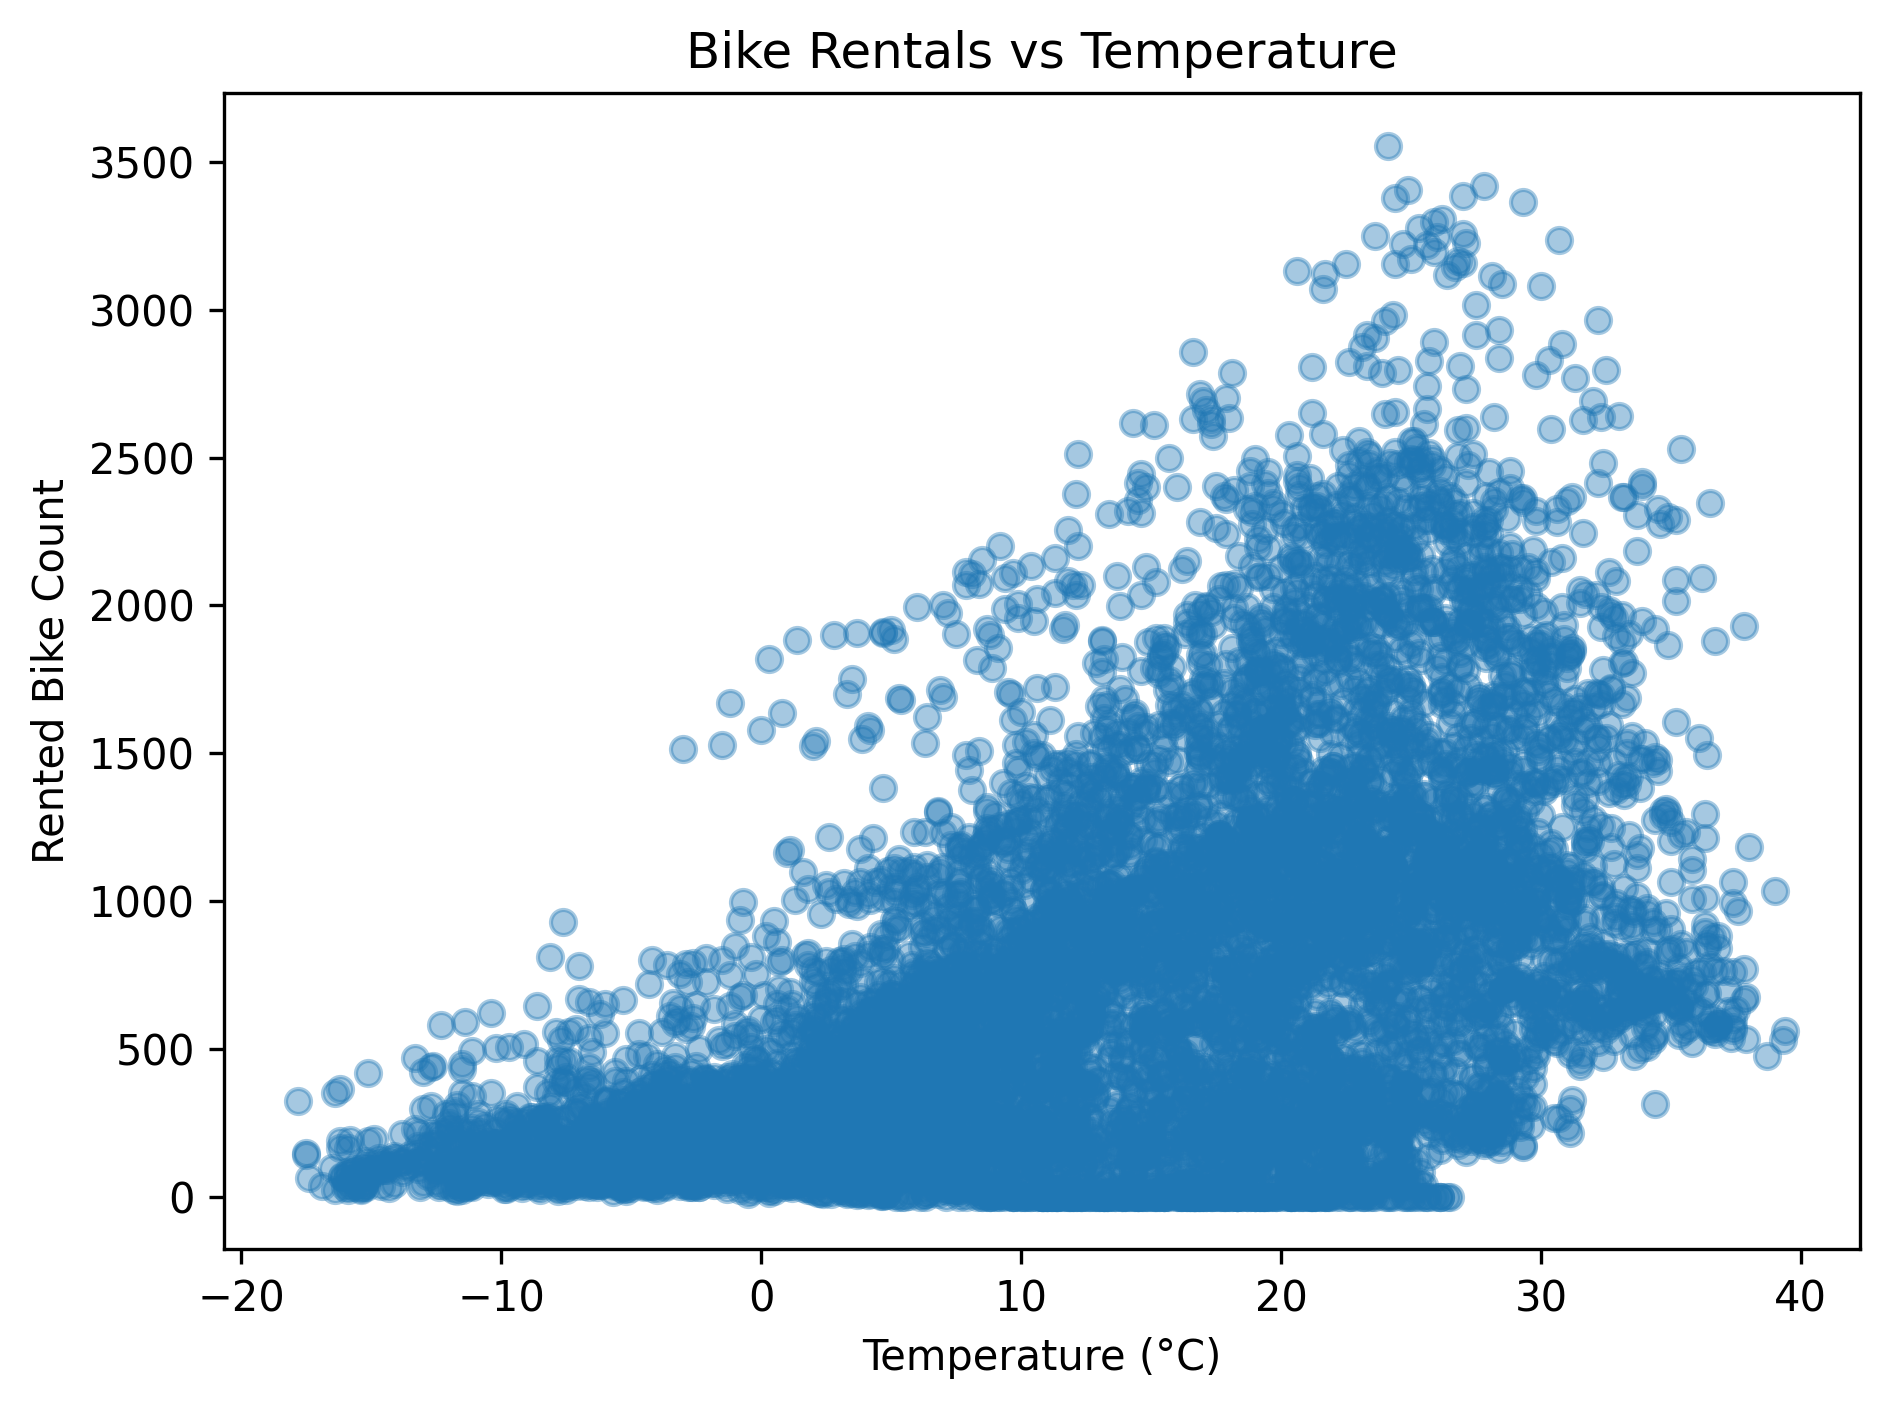
\includegraphics[width=\linewidth]{rentals_vs_temperature.png}
        \caption{Relationship between temperature and number of rented bikes.}
        \label{fig:rentals-temperature}
    \end{subfigure}\hfill
    \begin{subfigure}{0.48\textwidth}
        \centering
        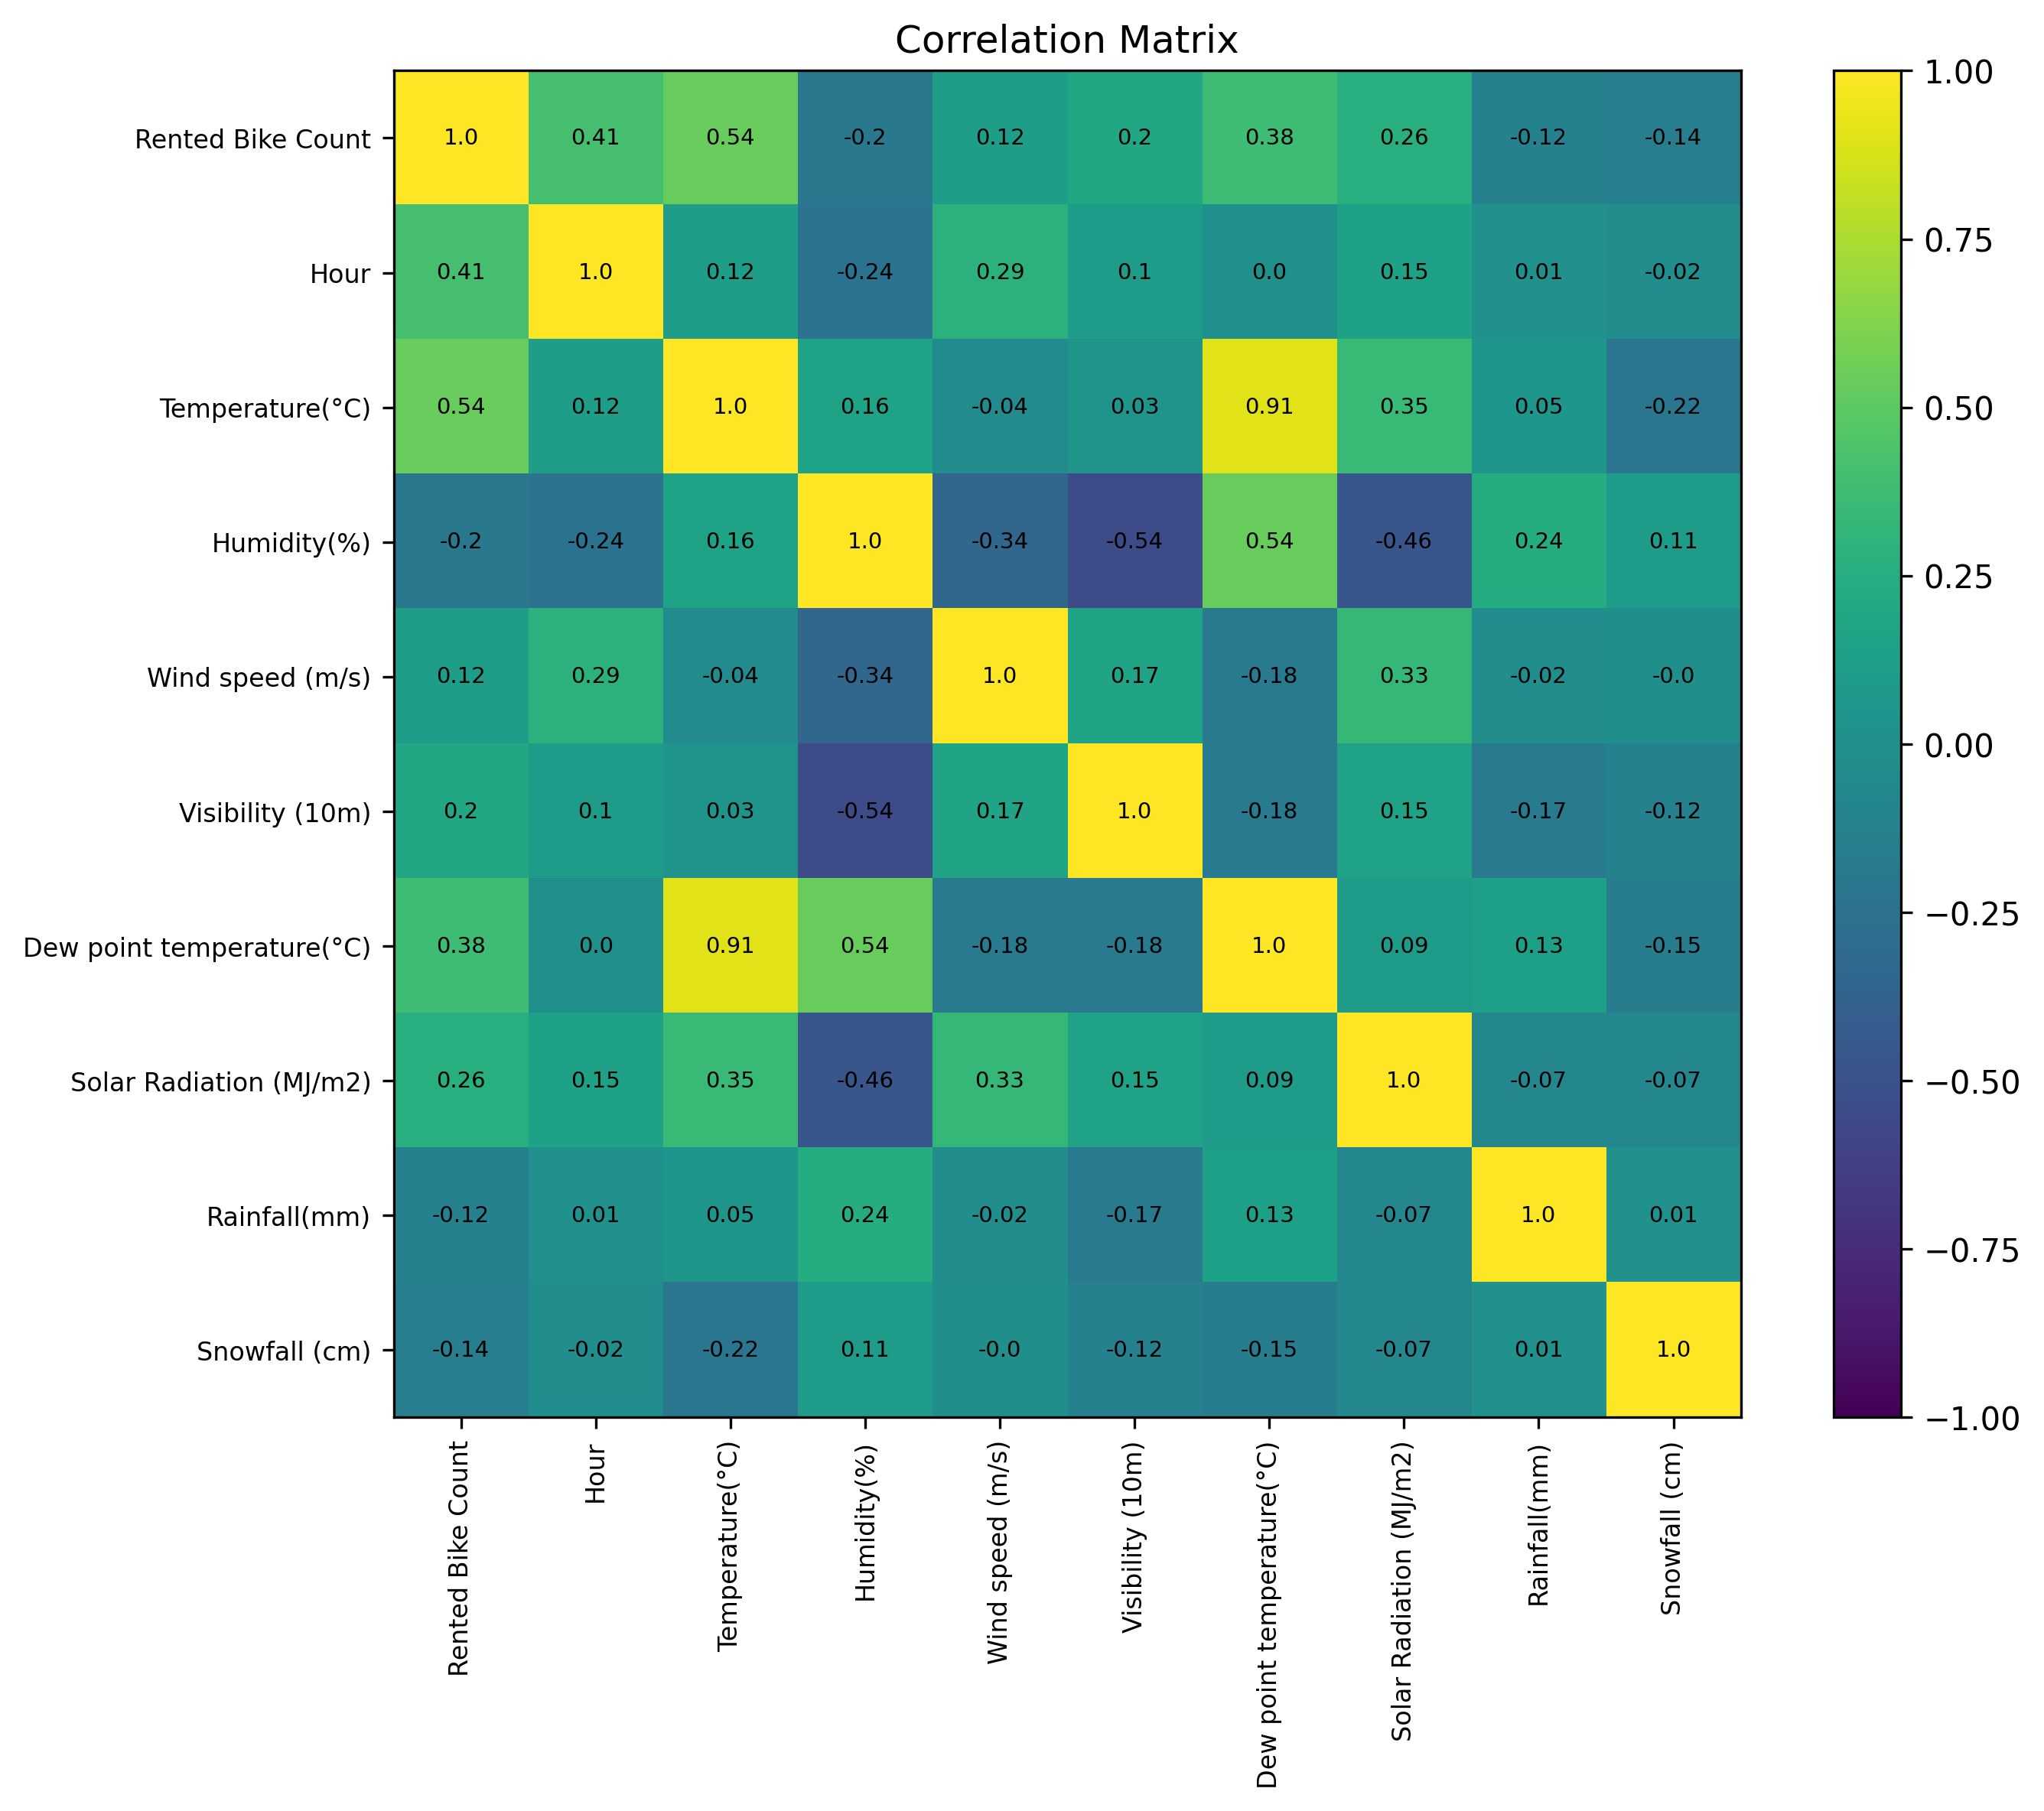
\includegraphics[width=\linewidth]{correlation_matrix.png}
        \caption{Correlation matrix of the numerical variables in the Seoul Bike Sharing dataset.}
        \label{fig:seoul-correlation}
    \end{subfigure}

    \caption{Exploratory analysis of the Seoul Bike Sharing dataset.}
    \label{fig:seoul-eda}
\end{figure}

\subsection{Preprocessing}

An initial check showed 295 observations with \emph{Rented Bike Count} equal to zero. All these observations correspond to days where \emph{Functioning Day} is \emph{No}. In these cases, zero does not represent a normal situation with no demand, but the fact that the bike sharing service was not operating. These observations were removed before modeling, because keeping them would introduce a different mechanism from the one we want to predict: when the service is closed, the number of rentals is necessarily zero, regardless of weather or time conditions.

Month and day of the week are extracted from the \emph{Date} variable. The \emph{Holiday} variable is converted into a binary indicator, while \emph{Seasons}, \emph{month}, \emph{day of the week}, and \emph{hour} are converted using dummy encoding, removing one reference category for each group. This gives a total of 52 features, which are then standardized using the mean and standard deviation.

For the stability experiment, the full dataset, which contains \textbf{8760 observations}, is not used. Instead, a sample of \textbf{1000 observations} is selected. This choice reduces computation time because the leave-one-out procedure requires fitting the model many times, each time after removing one observation. The sample of 1000 rows keeps enough data for the analysis while making the experiment more manageable.

The sample is split into training and test sets using the same proportion as in the synthetic experiments: $75\%$ of the data is used for training and the remaining $25\%$ for testing.

The experiment is repeated with \textbf{10 seeds}. This number is lower than for the synthetic data because the leave-one-out procedure takes more computation time on the real dataset. For Ridge, the same regularization values are used:

\begin{equation}
    \lambda \in \{0.001,\,0.01,\,0.1,\,1,\,10,\,100\}.
\end{equation}

This makes it possible to compare the results directly with those obtained on the synthetic data.

\subsection{Results on the Real Dataset}

The main results are summarized in Table~\ref{tab:real-results}. The table directly compares Least Squares and Ridge for different values of $\lambda$, considering both the test error and the average prediction change used as the empirical measure of stability.

Considering stability and Test MSE across the same values of $\lambda$ makes it possible to see more clearly where improved stability starts to come at the cost of predictive performance.

\begin{table}[ht]
    \centering
    \begin{tabular}{lcc}
        \toprule
        Model & Test MSE & Average prediction change \\
        \midrule
        Least Squares & 131678.6 & 1.7493 \\
        Ridge ($\lambda=0.001$) & 131618.9 & 1.7335 \\
        Ridge ($\lambda=0.01$)  & 131327.8 & 1.6782 \\
        Ridge ($\lambda=0.1$)   & 131066.1 & 1.4500 \\
        Ridge ($\lambda=1$)     & 166577.3 & 0.8775 \\
        Ridge ($\lambda=10$)    & 316903.2 & 0.6142 \\
        Ridge ($\lambda=100$)   & 395174.0 & 0.6882 \\
        \bottomrule
    \end{tabular}
    \caption{Comparison of Test MSE and average prediction change on the Seoul Bike Sharing dataset. Lower values of the second metric indicate greater stability.}
    \label{tab:real-results}
\end{table}

With very small values of $\lambda$, Ridge behaves very similarly to Least Squares. The most interesting case is $\lambda=0.1$: Test MSE stays almost at the same level as Least Squares, changing from $131678.6$ to $131066.1$, while the average prediction change decreases from $1.7493$ to $1.4500$, a reduction of about $17\%$. The average generalization gap also decreases, from $15664.7$ to $12327.4$. This value of $\lambda$ therefore gives the best trade-off observed on the real dataset.

As regularization increases further, the model becomes even less sensitive to the removal of single observations, but the error increases a lot. With $\lambda=10$, for example, the lowest average prediction change is obtained, equal to $0.6142$, but Test MSE increases to $316903.2$. In this case, greater stability is obtained at the cost of a large loss in predictive performance.

With $\lambda=100$, the prediction change also increases slightly again, from $0.6142$ to $0.6882$, while Test MSE increases further.

\begin{figure}[ht]
    \centering
    \begin{subfigure}{0.48\textwidth}
        \centering
        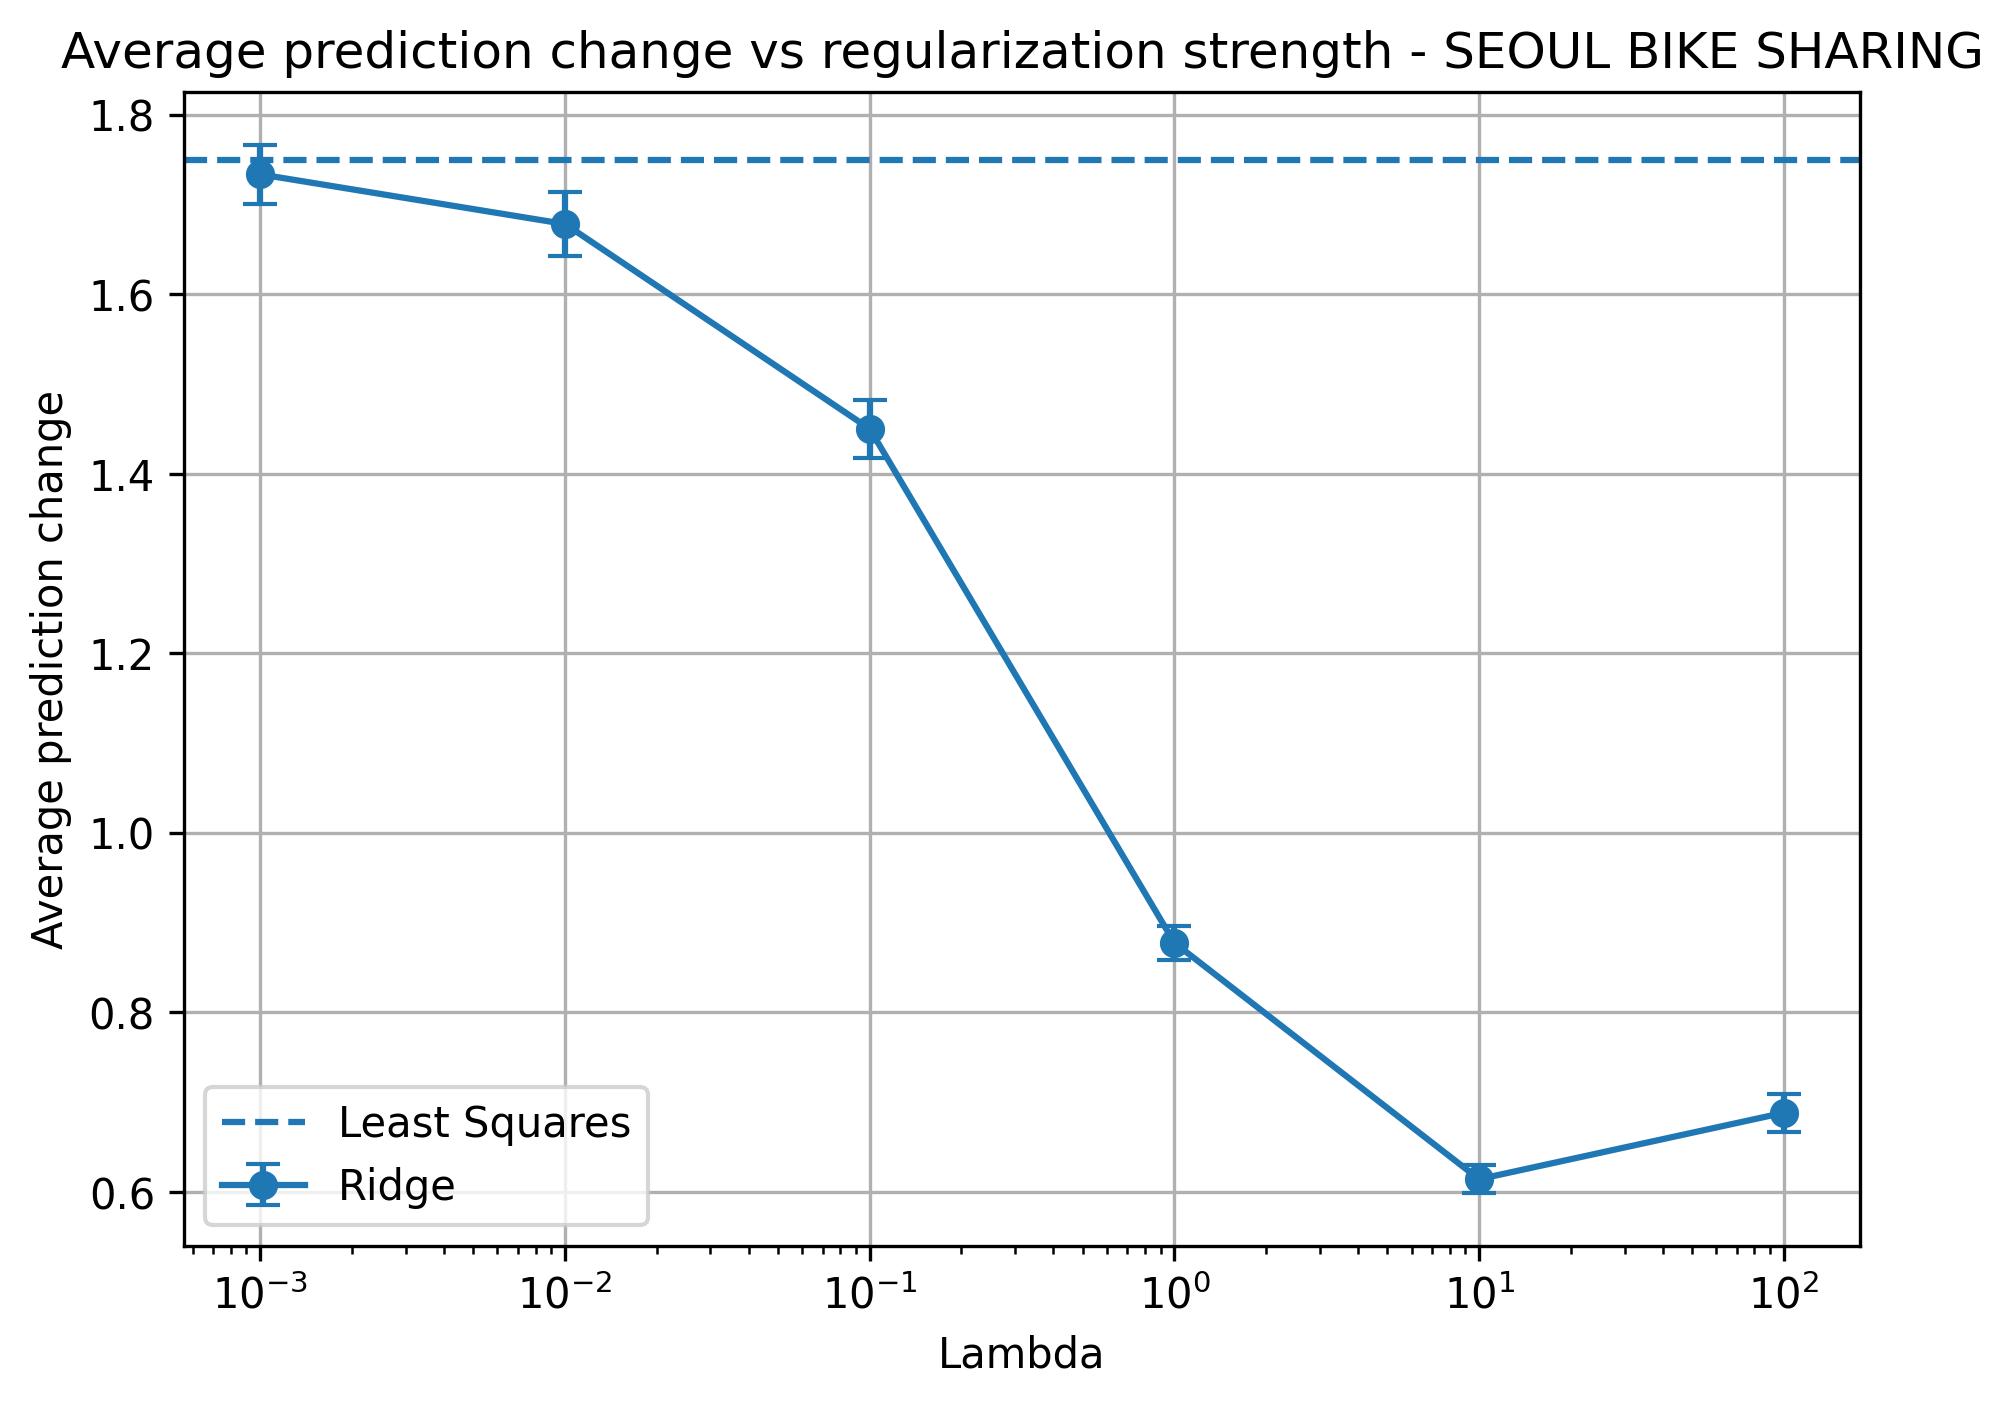
\includegraphics[width=\linewidth]{stability_vs_lambda_seoul_bike_sharing.png}
        \caption{Average prediction change for different values of $\lambda$.}
        \label{fig:real-stability}
    \end{subfigure}\hfill
    \begin{subfigure}{0.48\textwidth}
        \centering
        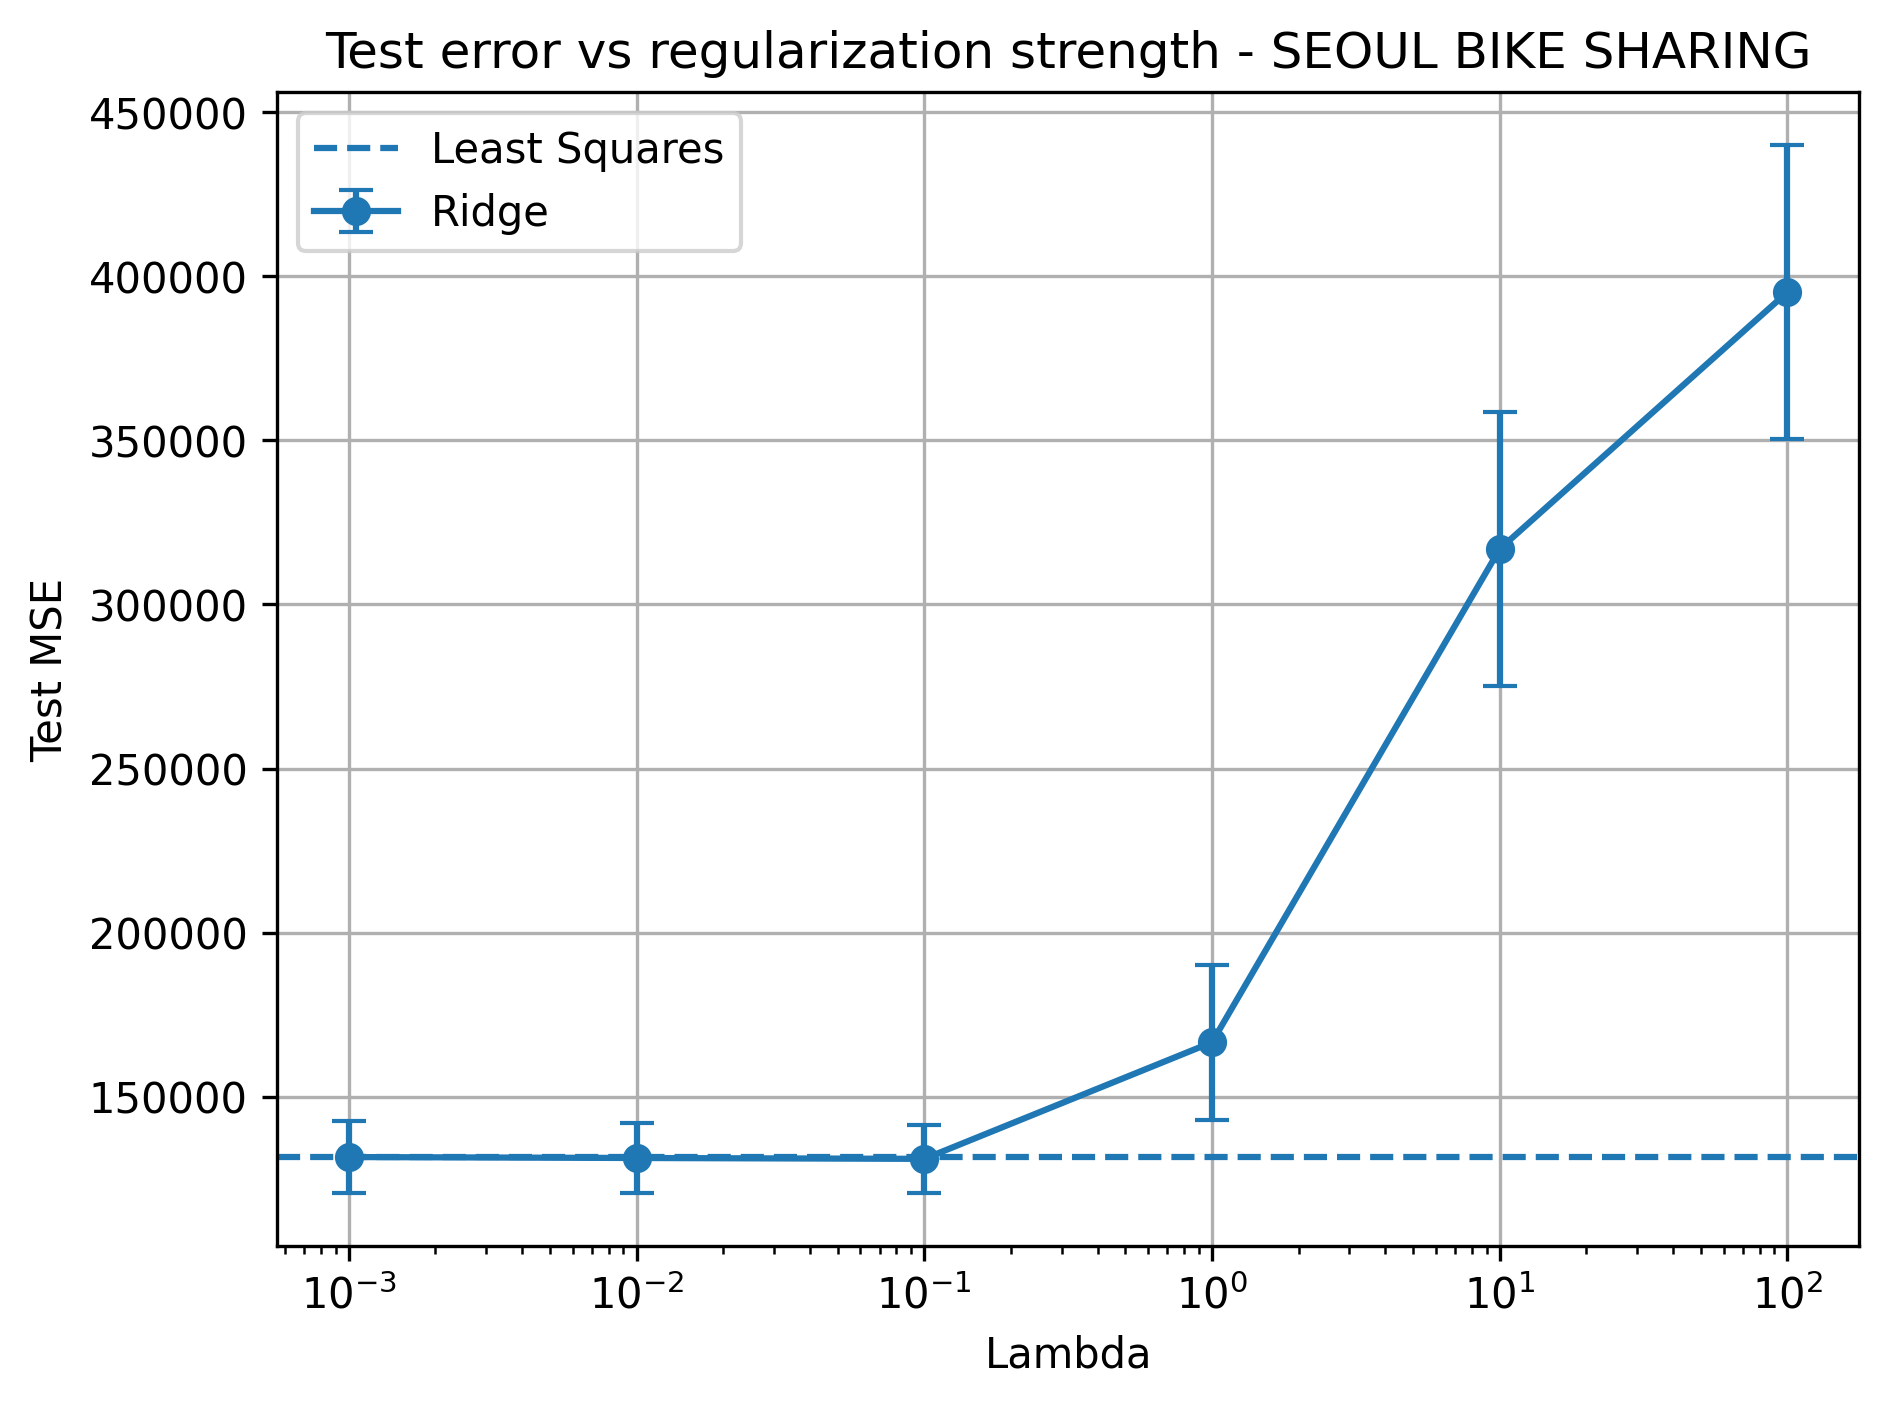
\includegraphics[width=\linewidth]{test_error_vs_lambda_seoul_bike_sharing.png}
        \caption{Test MSE for different values of $\lambda$.}
        \label{fig:real-test-error}
    \end{subfigure}
    \caption{Seoul Bike Sharing: empirical stability and predictive performance of Ridge for different levels of regularization.}
    \label{fig:real-results}
\end{figure}

Overall, the real dataset shows that moderate regularization, such as $\lambda=0.1$, improves stability without changing the test error in a meaningful way. Much larger values make the model more stable, but clearly worsen the predictions.

\section{Conclusions}

In this project, Least Squares and Ridge Regression were compared by looking at both prediction error and model stability when one observation is removed from the training set.

The experiments on synthetic data show that Ridge is especially useful when the predictors are correlated. In this case, moderate regularization, such as $\lambda=0.1$, reduces the change in predictions without increasing the error too much. When the predictors are independent, Least Squares is already quite stable and Ridge changes the model behavior only slightly. The experiments also show that both methods become more stable as the sample size increases.

A similar result is observed on the Seoul Bike Sharing dataset. With $\lambda=0.1$, Ridge reduces the average prediction change while keeping Test MSE very close to that of Least Squares. Larger values of $\lambda$ make the model even less sensitive to single observations, but strongly increase the prediction error.

Overall, the results show that Ridge can be useful for making the model more stable, but the benefit depends on the structure of the data and on the chosen value of $\lambda$. For this reason, stability and prediction error should be considered together.


\begin{thebibliography}{9}

\bibitem{bousquet2002stability}
O. Bousquet and A. Elisseeff,
\emph{Stability and Generalization},
Journal of Machine Learning Research, vol. 2, pp. 499--526, 2002.

\bibitem{hoerl1970ridge}
A. E. Hoerl and R. W. Kennard,
\emph{Ridge Regression: Biased Estimation for Nonorthogonal Problems},
Technometrics, vol. 12, no. 1, pp. 55--67, 1970.
\url{https://doi.org/10.1080/00401706.1970.10488634}

\bibitem{uci2020seoul}
UCI Machine Learning Repository,
\emph{Seoul Bike Sharing Demand} [Dataset], 2020.
\url{https://doi.org/10.24432/C5F62R}

\end{thebibliography}

\end{document}